\documentclass[12pt, a4paper]{article}
\usepackage[utf8]{inputenc}
\usepackage[spanish, es-tabla]{babel}
\usepackage{graphicx}
\usepackage{hyperref}
\usepackage{amsmath}
\usepackage{listings}
\usepackage{xcolor}
\usepackage{geometry}
\usepackage{enumitem}
\usepackage{titlesec}
\usepackage{booktabs}
\usepackage{longtable}
\usepackage{array}
\usepackage{tabularx}
\usepackage{tikz}
\usepackage{pdfpages}
\usepackage{float}
\usepackage{caption}
\usepackage{subcaption}
\usepackage{microtype}
\usepackage{tikz}
\usetikzlibrary{matrix, arrows.meta}
\graphicspath{{media/}}
\usetikzlibrary{positioning}
\geometry{margin=2.0cm}
\setlength{\parskip}{0.6em}
\setlength{\parindent}{0pt}

\titleformat{\section}{\large\bfseries}{\thesection}{1em}{}
\titleformat{\subsection}{\normalsize\bfseries}{\thesubsection}{1em}{}
\begin{document}
    \begin{titlepage}
        \centering
        \textbf{Universidad de La Habana \\
        Facultad de Matemática y Computación \\
        Año: 3ro\\
        Asignatura: Ingeniería de Software}\\[2cm]
        \begin{figure}[H]
            \centering
            
\includegraphics[width=0.45\textwidth]{logo.jpg}
        \end{figure}

        \vspace{1cm}

        {\LARGE \textbf{Seminario de Arquitecturas de Software:}}\\[0.5cm]
        {\large \textbf{Un Análisis Comparativo de Estilos Basados en Capas y Dominio}}

        \vspace{1.5cm}
        \textbf{Nombre de Equipo: SQLote}\\
        \begin{tabular}{ll}
            \textbf{Nombre y Apellidos} & \textbf{Pregunta} \\
            Ana Laura Oliva Avilés & 5 y 3\\
            Andriu Ferreyra Rodríguez & 6 \\
            Diana Martínez Almanza & 1 \\
            Yisell Velázquez Ochoa & 2 \\
            José Antonio Bello Cabrera & 4 \\
        \end{tabular}\\
        \href{https://github.com/AnaLauraOliva/matcom-bench-press}{Enlace al repositorio}

        \vfil
        Curso: 2026-2027
    \end{titlepage}
    \tableofcontents
    \newpage
    \section[Análisis de Trade-offs (Arquitectura N-Capas vs. Clean/Onion/Hexagonal)]{Pregunta 1: Análisis de Trade-offs (Arquitectura N-Capas vs. Clean/Onion/Hexagonal)}
        \subsection{Pregunta:}
        Un equipo de desarrollo está construyendo un sistema de gestión de inventario. Inicialmente, eligen una Arquitectura N-Capas tradicional por su simplicidad y familiaridad. Después de un año, el sistema se ha vuelto un “monolito” difícil de mantener, donde los cambios en la base de datos afectan la lógica de negocio y la interfaz de usuario, y las pruebas unitarias son lentas y frágiles.

        Con base en los principios de la Arquitectura Limpia y la Arquitectura Hexagonal, explique detalladamente qué error fundamental de acoplamiento se está cometiendo y cómo la introducción de la Regla de Dependencia (Martin) o el uso de Puertos y Adaptadores (Cockburn) resolverían estructuralmente este problema. ¿Cuál sería el impacto en la testabilidad y la capacidad de cambiar la base de datos de SQL Server a MongoDB sin afectar la lógica de negocio?

        \subsection{Error fundamental:}
        La arquitectura Limpia plantea que la estructura del sistema debe proteger las reglas de negocio de los detalles externos (Martin, 2018), mientras que la arquitectura hexagonal sostiene que la lógica de la aplicación debe poder desarrollarse y probarse de manera aislada de las tecnologías con las que interactúa como las interfaces de usuario y las bases de datos (Cockburn, 2005).

        Basándonos en los principios anteriores nos podemos dar cuenta de que el error fundamental que se cometió es que las dependencias entre las capas vinculan la lógica de negocio con los detalles de la base de datos, y como la UI depende de dicha lógica, también se ve afectada. 

        En una arquitectura N-Capas, la separación en capas no garantiza por sí sola un desacoplamiento efectivo. Si, como parece ser el caso, la lógica de negocio depende directamente de las clases concretas de acceso a datos, de consultas específicas de SQL Server o de estructuras que representan las tablas de la base de datos, los cambios en la persistencia pueden propagarse hacia la lógica de negocio y, posteriormente hacia la UI. Esto explicaría por qué el sistema se ha convertido en un monolito difícil de mantener pues existen dependencias que atraviesan las responsabilidades que deberían estar separadas.

        Seguidamente abordaremos la solución desde dos arquitecturas distintas: Arquitectura Limpia aplicando la Regla de Dependencia y Arquitectura Hexagonal usando Puertos y Adaptadores.

        \subsection{Alternativa A: Introducción de Regla de Dependencia}
        La Regla de Dependencia establecida por la Arquitectura Limpia plantea que las dependencias del código fuente deben dirigirse hacia el interior de la arquitectura (Martin, 2018), o sea, hacia las políticas y reglas de negocio de mayor nivel. Los elementos internos no deben depender de los elementos externos.

        Al aplicarla al problema debemos separar las responsabilidades en varios componentes: Entidades, Casos de Uso, Adaptadores de interfaz y la Infraestructura. La función que cada uno cumpliría en el sistema se puede observar en la \hyperref[tab:Tabla1.1]{Tabla 1.1}.

        \begin{table}[H]
            \centering

            \begin{tabular}{|l|p{10cm}|}
                \toprule
                Componente &Responsabilidad\\
                \midrule
                Entidades&Representan las reglas de negocio fundamentales\\
                Casos de Uso&Implementan las operaciones de la aplicación\\
                Adaptadores de interfaz&Transforman los datos entre los formatos utilizados por la aplicación y los que requieren los componentes externos, tales como la interfaz de usuario (UI) o la persistencia\\
                Infraestructura&Contiene los detalles técnicos, como la implementación del acceso a la base de datos, los controladores y los mecanismos concretos de comunicación\\
                \bottomrule

            \end{tabular}
            \caption*{Tabla 1.1: Componentes con sus responsabilidades al aplicar Regla de Dependencia}
            \label{tab:Tabla1.1}
        \end{table}
        
        Es necesario que las dependencias entre sus componentes respeten la Regla de Dependencia, de modo que las capas externas dependan de las abstracciones definidas hacia el interior de la arquitectura y no al contrario \hyperref[fig:Figura1.2]{(Figura 1.2)}. Así, la lógica de negocio permanece independiente de los detalles de implementación, haciendo posible que los componentes externos sean modificados sin afectar directamente las reglas fundamentales de la aplicación (Martin, 2018).

        \begin{figure}[H]
            \centering
            \begin{tikzpicture}
                \fill[blue!40] (0,0) circle(5.5cm);
                \fill[green!40] (0,0) circle(4cm);
                \fill[red!40] (0,0) circle(2.5cm);
                \fill[yellow!40] (0,0) circle(1cm);
                
                \draw[thick] (0,0) circle(1cm);
                \draw[thick] (0,0) circle(2.5cm);
                \draw[thick] (0,0) circle(4cm);
                \draw[thick] (0,0) circle(5.5cm);

                \node at (0,0) {Entidades};
                \node at (0,1.5)  {Casos de Uso};
                \node at (0,3) {Adaptadores de Interfaz};
                \node at (0,4.5){Infraestructura};

                \draw[-{Triangle}] (-4.75,0)--(-3.7,0);
                \draw[-{Triangle}] (-3.25,0)--(-2.20,0);
                \draw[-{Triangle}] (-1.75,0)--(-0.85,0);
            \end{tikzpicture}
            \caption*{Figura 1.2: Estructura propuesta para Arquitectura Limpia siguiendo Regla de Dependencia}
            \label{fig:Figura1.2}
        \end{figure}

        Sin embargo, en la práctica ocurre una aparente contradicción: si un caso de uso, como podría ser \texttt{ProductRegister}, necesita introducir un producto en la base de datos, en tiempo de ejecución debe invocar un método de un repositorio, si para esto dependiese de una clase concreta como \texttt{SqlServerProductRepository}, la dependencia del código fuente apuntaría hacia afuera, violando la Regla de Dependencia.

        Martin (2018) explica que esta aparente contradicción se resuelve usando el Principio de Dependencia Invertida, o sea, sacar provecho del polimorfismo dinámico para crear dependencias de código fuente que se oponen al flujo de control justamente en los puntos adecuados a lo largo del límite. Siguiendo nuestro ejemplo con \texttt{ProductRegister}, este define una abstracción, llamémosle \texttt{IProductRepository}, en el lado interno, y la infraestructura proporciona una implementación concreta \texttt{SqlServerProductRepository} que depende de esta interfaz y no al contrario. De esta manera, el flujo de control sigue siendo del caso de uso al repositorio, pero la dependencia del código fuente se inverte ya que la implementación externa apunta hacia la abstracción interna.

        \subsection*{Alternativa B: Uso de Puertos y Adaptadores}
        La arquitectura Hexagonal permite que una aplicación funcione y pueda probarse independientemente de los dispositivos externos, las interfaces de usuario y las bases de datos concretas (Cockburn, 2005).

        En este enfoque, el núcleo de la aplicación se comunica con el exterior usando puertos, que definen las operaciones y los contratos de interacción, y adaptadores, que traducen esos contratos a las particularidades de cada tecnología.

        La solución empleando esta arquitectura constaría de un núcleo de la aplicación que tendría las reglas de negocio y los casos de uso relacionados con la gestión del inventario, con puertos de entrada que permitirían solicitar las operaciones del sistema y puertos de salida que definirían los servicios externos que necesita la aplicación. Además, tendría adaptadores de entrada y de salida, los primeros traducirían las solicitudes recibidas de la UI, una API u otro mecanismo en el formato que espera el núcleo, mientras que los últimos implementarían los puertos de salida y traducirían las operaciones del núcleo a las instrucciones requeridas por la tecnología concreta de persistencia.

        La diferencia fundamental respecto a una arquitectura en la que las capas dependen directamente de las implementaciones concretas es que los componentes externos se conectan al núcleo mediante contratos definidos según las necesidades de la aplicación. Esto permite que se pueda sustituir un adaptador por otro sin tener que modificar el núcleo, siempre que el adaptador respete el contrato establecido (Cockburn, 2005).

        \subsection{Impacto en la testabilidad}
        La solución que implementa la Regla de Dependencia permite probar las entidades y los casos de uso sin necesitar que las pruebas dependan directamente de la base de datos o de la UI. Al depender de abstracciones, los componentes externos pueden sustituirse por implementaciones controladas durante las pruebas. Mientras, la solución con arquitectura Hexagonal hace explícita la posibilidad de probar la lógica de la aplicación sin depender de la UI ni de la base de datos ya que se pueden utilizar adaptadores de prueba o de bases de datos simuladas en memoria para comprobar el comportamiento de la aplicación sin tener que conectarse a la infraestructura real (Cockburn, 2005).

        Esto trae como consecuencia que las pruebas de las reglas de negocio puedan ejecutarse de manera aislada, rápida y predecible, sin que cada prueba unitaria tenga que inicializar la infraestructura real. Esto reduce la fragilidad causada por dependencias externas y facilita detectar errores en las reglas de dominio. Aún así, se requiere realizar pruebas de integración para verificar el correcto funcionamiento de los adaptadores con las tecnologías reales.

        \subsection{Cambiar de base de datos de SQL Server a MongoDB}
        Siempre que se cumplan las condiciones estructurales de los enfoques, la sustitución sería viable sin tener que modificar la lógica de negocio. Con Arquitectura Limpia, la lógica de negocio depende de abstracciones estables y no de clases o mecanismos propios de SQL Server, por lo que la implementación de persistencia puede sustituirse por otra que respete dichas abstracciones. Con Arquitectura Hexagonal, solo tendríamos que reemplazar el adaptador de persistencia de SQL Server por uno de MongoDB, conservando el puerto mediante el cual el núcleo solicita las operaciones de almacenamiento y recuperación.

        Sin embargo, como se está haciendo un cambio de una base de datos relacional a una documental, ambas pueden diferir en cuanto a representación de datos, consultas, transacciones y garantías de consistencia. Por ende, el nuevo adaptador debe traducir adecuadamente el modelo del dominio a la estructura de MongoDB y preservar el comportamiento requerido por el contrato. Es decir, el modelo relacional normalizado debe traducirse a documentos, las consultas SQL deben reescribirse con la API de MongoDB, y deben revisarse las transacciones y garantías de consistencia.

        Martin (2018) trata la base de datos como un plugin, con el objetivo de poder reemplazarla con cualquier otra variante de bases de datos SQL, bases de datos NoSQL, bases de datos basadas en archivos del sistema o cualquier otro tipo de tecnología de bases de datos que podríamos considerar necesaria en el futuro. Sin embargo, el propio autor reconoce que este reemplazo puede ser no trivial, pero que es posible.

        \section[Comparación de Estilos: La Simetría del Hexágono vs. la Jerarquía de las Capas]{Ejercicio 2: Comparación de Estilos: La Simetría del Hexágono vs. la Jerarquía de las Capas}
        \subsection{Pregunta:}
        La Arquitectura Hexagonal de Cockburn y la Arquitectura Onion de Palermo comparten el objetivo de aislar el núcleo de negocio, pero utilizan representaciones visuales y metáforas radicalmente diferentes (un hexágono simétrico frente a capas concéntricas).

        Analice en profundidad qué problema conceptual resuelve la simetría de la representación hexagonal que una representación de capas apiladas (como la de Onion o la N-Capas tradicional) no logra transmitir de forma intuitiva. ¿Cómo se traduce el concepto de ``Puerto y Adaptador'' en la práctica de definir interfaces en las capas internas de la Arquitectura Onion? ¿Por qué Cockburn afirma que el hexágono no tiene seis lados por una razón numérica, sino para eliminar la asimetría izquierda-derecha o arriba-abajo?

        \subsection{Breve descripción de ambas arquitecturas}
        La arquitectura Hexagonal, también conocida como Arquitectura de Puertos y Adaptadores busca crear sistemas débilmente acoplados, donde la lógica de negocio (dominio) esté completamente aislada de los detalles externos como bases de datos, interfaces de usuario o APIs.
        
        Puertos: Son interfaces definidas por la propia aplicación. Representan los puntos de entrada y salida a través de los cuales el núcleo se comunica con el exterior.
        
        Adaptadores: Son implementaciones completas específicas de cada tecnología.
        
        La regla fundamental es que las dependencias siempre apuntan hacia el centro. El núcleo de la aplicación no conoce ni depende de los adaptadores.

        La arquitectura Onion fue propuesta por Jeffrey Palermo con el objetivo de resolver los problemas de acoplamiento y separación de responsabilidades de las arquitecturas tradicionales en capas. Su idea central es que el código puede depender de capas más internas pero no de capas más externas. Palermo define 4 anillos concéntricos principales (de adentro hacia afuera):
        \begin{itemize}
            \item Capa de dominio
            \item Capa de servicios de dominio
            \item Capa de servicios de aplicación
            \item Capa de infraestructura
        \end{itemize}

        \subsection{Simetría de la representación hexagonal y el problema conceptual que resuelve (que una representación de capas apiladas no transmite intuitivamente)}
        La simetría hexagonal elimina la jerarquía implícita entre los actores externos y convierte al núcleo en protagonista, no en una capa más de una pila.

        El problema de la jerarquía implícita en las capas apiladas puede ser visualizado en la \hyperref[fig:Figura2.1]{Figura 2.1}
        \begin{table}[H]
            \centering
            \begin{tikzpicture}
                \matrix(capas)[
                    matrix of nodes,
                    nodes={draw, minimum width=4cm, minimum height=0.8cm, anchor=center, align=center},
                    row sep = -\pgflinewidth
                ]{
                    Presentación \\
                    Aplicación\\
                    Dominio\\
                    Infraestructura\\
                    Base de Datos\\
                };

                \node[right=5mm of capas-1-1]{arriba};
                \draw[-{Triangle}]([xshift=5mm]capas-1-1.east) -- ([xshift=0mm]capas-1-1.east);

                \node[right=5mm of capas-5-1]{abajo};
                \draw[-{Triangle}]([xshift=5mm]capas-5-1.east) -- ([xshift=0mm]capas-5-1.east);
            \end{tikzpicture}
            \caption{Figura 2.1: Problema de la jerarquía implícita en las capas apiladas}
            \label{fig:Figura2.1}
        \end{table}

        La verticalidad no es inocente. Impone varias ideas falsas:
        \begin{itemize}
            \item Arriba = ``más cerca del usuario, más importante o más superficial''
            \item Abajo = ``más fundamental o más estable''
            \item Flujo vertical: la petición ``baja'' y la respuesta ``sube''
        \end{itemize}
        Ninguna de estas jerarquías existe en el dominio del problema. La arquitectura Onion lo corrige parcialmente \hyperref[fig:Figura2.2]{(Figura 2.2)}.
        \begin{table}[H]
            \centering
            \begin{tikzpicture}
                \draw[thick](0,0) circle (3cm);
                \draw[thick](0,0) circle (2cm);
                \draw[thick](0,0) circle (1cm);

                \node at (0,0) {Dominio};
                \node at (0,1.4) {Aplicación};
                \node at (0,2.4) {Infraestructura};
            \end{tikzpicture}
            \caption*{Figura 2.2: Estructura de la arquitectura Onion}
            \label{fig:Figura2.2}
        \end{table}

        Pero sigue siendo radial-jerárquico. La verticalidad sugiere un conocimiento asimétrico que no debería existir.

        El hexágono no tiene vértice superior ni inferior privilegiado. No hay actores externos ``por encima'' ni ``por debajo'' del núcleo. Todos están a la misma distancia conceptual. Esta es una idea poderosa que las capas no pueden expresar con naturalidad. El hexágono representa esta ``simetría de ignorancia'' de forma visual inmediata: todos los puertos están en el mismo borde, a la misma distancia, sin jerarquía.

        En una arquitectura como N-Capas la dirección de dependencia y la dirección de flujo coinciden. En Hexagonal se separan:

        La dirección de dependencia es siempre hacia adentro: los adaptadores dependen de los puertos, el núcleo no depende de nada.

        La dirección de flujo puede ser en cualquier dirección: el núcleo puede invocar a un adaptador secundario (salida) y un adaptador primario puede invocar al núcleo (entrada).

        Esta separación es imposible de representar con una pila vertical sin ambigüedad. La pila sugiere que el flujo y la dependencia son lo mismo. El hexágono con su simetría radial permite que el flujo vaya en cualquier dirección mientras que la dependencia siempre apunta al centro.

        \subsection{Traducción del concepto de ``Puerto y Adaptador'' en la práctica de definir interfaces en las capas internas de la Arquitectura Onion}
        En la arquitectura Hexagonal el concepto de puerto es explícito y tiene un lugar físico en el diagrama: el borde del hexágono. En Onion no existe una capa llamada ``puertos'', pero el concepto no desaparece: se disuelve dentro de las capas internas. Mientras que los adaptadores viven todos en la capa más externa: Infrastructure.

        Un puerto se convierte en cualquier interfaz definida en una capa interna que es implementada por una capa externa.

        \subsubsection*{Puertos secundarios → interfaces en DomainServices}
        En Hexagonal un puerto secundario es una interfaz que el núcleo usa para salir hacia el exterior. En Onion esa interfaz se coloca en la capa de DomainServices, que es la capa inmediatamente exterior al dominio puro.

        \subsubsection*{Puertos primarios → interfaces en ApplicationsServices}
        En Hexagonal un puerto primario es la interfaz que define cómo el exterior puede invocar al núcleo. En Onion, esa interfaz se coloca en la capa de ApplicationsServices, que es la capa que orquesta los casos de uso.

        En Hexagonal los puertos y adaptadores están agrupados, en Onion están distribuidos.

        \subsection{La razón no es numérica: eliminar la asimetría izquierda-derecha o arriba-abajo}
        La elección de Cockburn responde a una necesidad puramente gráfica y conceptual: eliminar las connotaciones jerárquicas que imponen las representaciones lineales. El hexágono al tener múltiples lados permite distribuir los puertos perimetralmente sin sugerir que unos sean más importantes que otros.

        Cockburn (2005) explica: El hexágono no es un hexágono porque el número seis sea importante, sino más bien para permitir que quienes hacen el dibujo tengan espacio para insertar puertos y adaptadores según lo necesiten, sin verse limitados por un dibujo estratificado unidimensional. El término arquitectura hexagonal proviene de este efecto visual.

        Al usar un hexágono ya no hay una ``capa superior'' o una ``capa inferior''. Todos los actores externos (usuarios, tests, bases de datos, servicios de mensajería) quedan en el perímetro, a la misma distancia conceptual del núcleo. Esto transmite visualmente que todos los puertos son de naturaleza similar y que ninguno es intrínsecamente más fundamental que otro.

        Según Cockburn (2005): La asimetría que hay que explotar no es la que existe entre los lados izquierdo y derecho de la aplicación, sino entre el interior y el exterior de la aplicación. La regla que se debe obedecer es que el código perteneciente a la parte interior no debe filtrarse hacia la parte exterior.

        \section[Aplicación de DDD y Bounded Context en un Dominio Complejo]{Pregunta 3: Aplicación de DDD y Bounded Context en un Dominio Complejo}
        \subsection{Pregunta}
        Una empresa de seguros necesita desarrollar un sistema para gestionar pólizas de automóviles. El sistema debe interactuar con un departamento de siniestros, un sistema de facturación de primas y una aplicación para que los ajustadores de seguros evalúen daños en el lugar del accidente. Cada uno de estos subsistemas tiene su propia terminología y preocupaciones (ej: ``póliza'' para un actuario es un contrato con cláusulas, para facturación es una fuente de ingresos, y para un ajustador es un número de referencia).

        Basado en los conceptos de Domain-Driven Design (Evans) y Bounded Context (Richards \& Ford), explique cómo dividiría este sistema en varios contextos delimitados. ¿Cómo evitaría que el modelo de “Póliza” se contamine con detalles de siniestros o facturación? ¿Cómo se comunicarían estos contextos de manera desacoplada? Relacione esta solución con la implementación de una Arquitectura Orientada al Dominio (como Onion o Clean) y la creación de un Adaptador de Servicio para la comunicación externa, tal como se describe en la Guía de Arquitectura N-Capas.

        \subsection{División del problema en Bounded Contexts}
        
        Richards y Ford (2020) plantean que algunas pautas que ayudan a los arquitectos a encontrar los límites adecuados son el propósito (el límite de cada contexto debe definirse por su dominio y cohesión funcional), transacciones (los contextos delimitados son flujos de negocio, y las entidades que cooperan en una transacción suelen señalar un buen límite de servicio) y la coreografía (si un conjunto de contextos logra un buen aislamiento de dominio pero exige demasiada comunicación para funcionar, conviene reagruparlos en un servicio mayor para reducir el costo de coordinación).

        La misma idea de Bounded Contexts es planteada por de la Torre, Zorrilla, Ramos y Calvarro (2010), solo que bajo el nombre de módulos. Plantean que un principio aceptado por la industria es el hecho de que el código debe tener un alto nivel de cohesión y un bajo nivel de acoplamiento, además, debido a que la cohesión empieza en el nivel de las clases y los métodos, pero que también puede aplicarse a nivel de módulo, recomiendan agrupar las clases relacionadas en módulos de forma que se proporcione la máxima cohesión posible. Mencionan que existen varios tipos de cohesión, pero que dos de las más utilizadas son ``Cohesión de Comunicaciones'' (partes de un módulo que operan sobre los mismos conjuntos de datos) y ``Cohesión Funcional'' (se consigue cuando todas las partes de un módulo realizan una tarea o conjunto de tareas funcionales bien definidas). El uso de módulos en un diseño es una buena forma de aumentar la cohesión y disminuir el acoplamiento. El nombre de cada módulo debe formar parte del ``Lenguaje Ubicuo'' de DDD y en la comunicación entre módulos se hace por medio de una interfaz (por ejemplo, un Servicio DDD).

        Para tratar este problema, como cada subsistema (la gestión de seguros, el departamento de siniestros, el sistema de facturación de primas y la aplicación para que los ajustadores de seguros evalúen daños en el lugar del accidente) tiene sus propias terminologías y preocupaciones lo dividimos en cuatro Bounded Contexts siguiendo las pautas anteriormente mencionadas: Gestión de pólizas, gestión de siniestros, facturación de primas y evaluación de daños. En caso de que dentro de uno de los contextos antes definidos existan modelos y reglas de negocio diferentes, se pueden crear otros contextos, pero para este caso asumimos que esto no ocurre.

        El contexto Gestión de Pólizas se encarga de crear y administrar las pólizas de automóviles, incluyendo, por ejemplo, sus cláusulas, coberturas, condiciones y períodos de vigencia. Por otro lado, el contexto Gestión de Siniestros se ocupa de registrar los accidentes, tramitar las reclamaciones y determinar su estado.

        También tenemos el contexto Facturación de Primas que gestiona el cálculo de las primas, la emisión de las facturas y el control de los pagos. Por último, el contexto Evaluación de Daños permite a los ajustadores registrar los daños del vehículo, recopilar evidencias y elaborar informes desde el lugar del accidente.

        Cabe destacar que las funcionalidades asignadas a cada contexto son puramente ilustrativas debido a que no se especifica en detalle los requisitos de cada subsistema.

        \subsection{Evitando la contaminación del modelo ``Póliza''}

        Cada uno de los contextos tiene su propio modelo Póliza, que se adapta a sus necesidades y responsabilidades, es decir, mantiene únicamente los datos y las reglas de negocio que necesita. Estos modelos son independientes entre sí y comparten un IdPóliza para correlacionar la póliza entre contextos, pero solo eso. La \hyperref[tab:Tabla3.1]{Tabla 3.1} define los modelos Póliza de cada contexto.

        \begin{table}[H]

            \begin{tabular}{|c|c|p{5cm}|}

                \toprule

                Nombre&Contexto&Función\\

                \midrule

                Póliza&Gestión de Pólizas&Contrato entre el cliente y la aseguradora\\

                Póliza\_Siniestros&Gestión de Siniestros&Contrato que permite comprobar si el siniestro está cubierto y bajo qué condiciones\\

                Póliza\_Primas&Facturación de Primas&Fuente de ingresos que determina las obligaciones de pago del cliente\\

                Póliza\_Eval\_Daños&Evaluación de Daños&Número de referencia para localizar la información necesaria\\

                \bottomrule

            \end{tabular}

            \caption*{Tabla 3.1: Propuesta que ilustra cómo cada contexto tiene su propio modelo Póliza}

            \label{tab:Tabla3.1}

        \end{table}

        La comunicación entre contextos se lleva a cabo mediante interfaces bien definidas, evitando que dependan directamente de los modelos internos de los demás. Para ello, cada contexto expone únicamente las operaciones y los datos que los demás necesitan para colaborar con él, de forma tal que puedan intercambiar la información necesaria sin conocer cómo implementan internamente sus modelos. Además, se utiliza una Anticorruption Layer (ACL) (Evans, 2003) por parte del contexto consumidor para traducir la información recibida al modelo y la terminología del contexto correspondiente sin correr el riesgo de que un modelo contamine al otro.

        Precisamente así se relacionan los modelos Póliza de cada uno de los contextos evitando que se contaminen en el proceso. Con esto, se preserva la independencia de los modelos y se evita que el modelo principal Póliza incorpore detalles específicos de siniestros o facturación.

        \subsection{Comunicación entre contextos}

        La comunicación entre contextos puede ser de dos formas: síncrona y asíncrona.

        Primero centrémonos en la comunicación síncrona: Para validaciones que requieran una respuesta inmediata del proveedor antes de que el consumidor pueda continuar, como comprobar la vigencia de una póliza, verificar si un siniestro está cubierto o confirmar que un IdPóliza corresponde a una póliza válida. En estos casos el contexto consumidor invoca una operación del contrato público del proveedor y queda bloqueado a la espera de la respuesta. 
        
        Para ilustrarlo hagamos que nuestro contexto Gestión de Siniestros registre una reclamación: antes de decidir si tramita o rechaza el siniestro, necesita saber si la póliza está vigente y si el tipo de siniestro está cubierto. Para ello invoca una operación del contrato público de Gestión de Pólizas, digamos \texttt{checkCoverage(IdPóliza, accidentType)}, y espera la respuesta. Gestión de Póliza evalúa con sus propias reglas de negocio la vigencia y las condiciones de cobertura y devuelve el resultado. Gestión de Siniestros traduce esa respuesta a su propio modelo Póliza\_Siniestros por medio de una Anticorruption Layer y continúa con la tramitación. Se mantiene que el consumidor no conoce la implementación interna del proveedor, solo la operación expuesta y el formato de su respuesta.

        En cuanto a la asíncrona Richards y Ford (2020) plantean que los arquitectos a menudo usan eventos y mensajes, los cuales internamente usan una arquitectura dirigida a eventos o EDA. De la Torre et al. (2010) dicen que es un patrón de arquitectura que promociona fundamentalmente el uso de eventos como hilo conductor principal de ejecución de cierta lógica del Dominio.

        Un evento puede definirse como ``un cambio significativo de estado'' por lo que un sistema que implemente esta lógica podría tratar este cambio de estado como un evento que se pueda producir, detectar y consumir por varios componentes dentro de la arquitectura.

        En el problema, se puede usar comunicación asíncrona para añadir una póliza: se publica el evento issuedPolicy que contiene idPóliza y los datos mínimos para que otros contextos reaccionen, por ejemplo, Facturación de Primas se suscribe a ese evento y, al recibirlo, calcula la prima y genera la factura correspondiente. Al igual que con síncrona, el consumidor no conoce los modelos internos del proveedor, solo conoce el contrato del evento y, si necesita traducir información a su propio modelo, interpone una Anticorruption Layer.

        \subsection{Relación con arquitecturas orientadas al dominio y creación de Adaptador de Servicio}
        Esta solución se relaciona con la implementación de una arquitectura como Onion o Clean, que son orientadas al dominio, pues ambas buscan separar la lógica de negocio de los detalles de infraestructura y de los sistemas externos. Así, cada contexto mantendría su modelo y sus reglas de negocio independientes, mientras que la comunicación con otros sistemas se produciría por medio de interfaces y componentes externos a la lógica central del dominio.

        Para finalizar, abordemos la creación de un Adaptador de Servicio para la comunicación externa.

        Un adaptador tiene como función el permitir la comunicación entre dos componentes o sistemas con interfaces diferentes, transformando las solicitudes, los datos o las respuestas para que puedan interactuar sin tener que modificar su comportamiento interno (Evans, 2003).

        El adaptador encapsularía los detalles de la comunicación con el sistema externo, como el protocolo utilizado, el formato de los mensajes y la transformación de los datos. De esta forma, no tendrían que ser implementados por los contextos que necesiten comunicarse.

        \section[Evaluación de la Inversión de Dependencias en la Práctica]{Pregunta 4: Evaluación de la Inversión de Dependencias en la Práctica}

        \subsection{Pregunta}
        Un equipo de desarrollo está trabajando en un sistema de gestión de pedidos. La lógica de negocio principal se encuentra en una clase \texttt{OrderProcessor} que, para completar su tarea, necesita comunicarse con un servicio externo de validación de direcciones. La implementación actual tiene una dependencia directa: \texttt{OrderProcessor} instancia y llama directamente a la clase \texttt{AddressValidatorService}, que a su vez depende de una librería HTTP específica para comunicarse con el servicio externo.

        Con base en los principios de la Inversión de Dependencias (Martin) y la Regla de Dependencia (Martin), analice y responda:

        \begin{enumerate}[label=\alph*)]
            \item ¿Por qué esta dependencia directa viola los principios fundamentales de las arquitecturas Hexagonal, Limpia y Onion? Explique específicamente qué dirección deberían tener las dependencias del código fuente y por qué la implementación actual no la cumple.

            \item Rediseñe la interacción entre \texttt{OrderProcessor} y \texttt{AddressValidatorService} para que se alinee con los principios de estas arquitecturas. Defina claramente qué componente (interfaz) debe residir en el núcleo de la aplicación y qué componente debe residir en la capa de infraestructura o en el exterior del hexágono. Justifique su diseño basándose en el principio de que ``los detalles deben depender de las abstracciones''.

            \item Explique cómo este nuevo diseño permite que la lógica de negocio (\texttt{OrderProcessor}) sea probada de forma aislada, sin necesidad de realizar llamadas HTTP reales al servicio externo, y sin depender de la librería HTTP subyacente. ¿Qué implicaciones tiene este diseño para la mantenibilidad y la capacidad de cambiar el proveedor de validación de direcciones en el futuro?
        \end{enumerate}

        \subsection{Breve introducción a la Inversión de Dependencias y la Regla de Dependencia}
        
        Martin (2018) expone en su libro ``Arquitectura Limpia'' un conjunto de reglas y principios para diseñar software mantenible, testeable e independiente de frameworks y herramientas externas.

        La regla de la dependencia es el principio fundamental que hace funcionar a la arquitectura limpia, Martin (2018) la define de forma muy clara:

        ``Las dependencias del código fuente solo pueden apuntar hacia adentro, hacia políticas de alto nivel''.

        En la práctica, esto significa que nada en un círculo interno puede saber absolutamente nada sobre algo en un círculo externo; ni siquiera puede mencionar el nombre de una función, clase o variable declarada afuera.

        El principio de inversión de dependencias (DIP) es el quinto principio de SOLID y actúa como la base para lograr la Regla de la Dependencia. Martin (2018) lo resume en una idea:

        “El Principio de Inversión de Dependencias (DIP) nos dice que los sistemas más flexibles son aquellos en los que las dependencias del código fuente se refieren solo a abstracciones, no a concreciones.”

        Esta idea se desglosa en dos puntos clave. Los módulos de alto nivel no deben depender de los de bajo nivel: ambos deben depender de abstracciones. La lógica de negocio (alto nivel) no debe estar acoplada a detalles como la base de datos o la interfaz de usuario (bajo nivel). Las abstracciones no deben depender de los detalles: son los detalles (implementaciones concretas) los que deben depender de las abstracciones.

        \subsection{Razón por la cual la dependencia interna viola los principios fundamentales de las arquitecturas Hexagonal, Limpia y Onion}

        Las tres arquitecturas (Limpia, Hexagonal y Cebolla) comparten exactamente la misma filosofía central: proteger la lógica de negocio (el dominio) de los detalles de infraestructura (como bases de datos, frameworks o APIs externas). Al tener una dependencia directa, se violan sus principios de la siguiente manera:
        \begin{itemize}   
            \item Arquitectura Limpia (Clean Architecture): Viola directamente la Regla de la Dependencia. Según Martin, las dependencias del código fuente solo pueden apuntar hacia adentro. En este caso, OrderProcessor (que debería estar en el círculo interno de Casos de Uso) está apuntando hacia afuera al conocer y crear una instancia de AddressValidatorService (que pertenece al círculo externo de Adaptadores/Infraestructura).
            \item Arquitectura Hexagonal (Puertos y Adaptadores): En este patrón, el núcleo de la aplicación debe exponer puertos (interfaces) para comunicarse con el exterior, y los agentes externos actúan como adaptadores. Aquí, OrderProcessor no está usando un puerto abstracto, sino que está acoplado directamente a un adaptador concreto AddressValidatorService. El núcleo de negocio está ``sabiendo'' cómo se comunica con el exterior.
            \item Arquitectura Onion (Cebolla): Esta arquitectura establece que el Dominio y los Servicios de Aplicación (el centro) no deben tener dependencias hacia la Infraestructura (las capas externas). Al acoplar OrderProcessor a un servicio que usa HTTP, se está contaminando la capa de dominio con detalles tecnológicos (la red, el protocolo HTTP).
­        \end{itemize}

        \subsection{Dirección que deberían tener las dependencias del código fuente. Razón por la que la implementación actual no la cumple}
        
        Las dependencias del código fuente deben apuntar siempre hacia adentro (hacia el dominio o lógica de negocio).

        Esto significa que:
        \begin{itemize}
            \item El código de alto nivel (reglas de negocio, entidades, casos de uso) no debe saber nada sobre el código de bajo nivel (controladores, bases de datos, servicios externos, HTTP).
            \item Si el módulo de alto nivel (OrderProcessor) necesita usar funcionalidades del bajo nivel (AddressValidatorService), el bajo nivel debe depender del alto nivel, y no al revés. Esto se logra mediante el uso de abstracciones (interfaces) que pertenecen al núcleo.
        \end{itemize}
        La implementación actual no cumple con esta dirección porque el código fuente de OrderProcessor menciona explícitamente (instancia) a la clase AddressValidatorService.

        \subsection{Rediseño de la interacción}

        Para alinear el diseño con los principios de estas arquitecturas la clave está en invertir la flecha de dependencia creando una abstracción (interfaz) que sea propiedad del núcleo de negocio.

        La interfaz (puerto): se crea una interfaz llamada IAddressValidator que contiene solo la firma del método que el negocio necesita, por ejemplo boolean isValidAddress(Address address).

        Consumidor: la clase OrderProcessor. Ahora esta clase solo depende de esta interfaz. No sabrá que existe algo llamado AddressValidatorService, ni una librería HTTP.

        Lo que reside en la capa de infraestructura sería la implementación (adaptador): la clase AddressValidatorService y la librería HTTP.


        El Flujo de Dependencias (Invertido)
        \begin{enumerate}
            \item OrderProcessor (Núcleo) depende de IAddressValidator (Núcleo).
            \item AddressValidatorService (Infraestructura) depende de  IAddressValidator (Núcleo).
            \item AddressValidatorService (Infraestructura) depende de Librería HTTP (Exterior).
        \end{enumerate}
        Este diseño está justificado por el DIP ya que los detalles dependen de las abstracciones: el protocolo HTTP, el formato JSON, y la URL del servicio externo son detalles. La clase AddressValidatorService es un detalle de implementación. Al implementar la interfaz IAddressValidator es el detalle (el servicio externo) el que se adapta al contrato exigido por el núcleo. La inversión del control: antes, el negocio (alto nivel) dependía de la infraestructura (bajo nivel). Ahora, ambas capas dependen de la abstracción (IAddressValidator). El negocio dicta qué necesita, sin importar cómo se hace.

        De esta manera, las dependencias del código fuente apuntan hacia adentro, protegiendo las reglas de negocio y dejando los frameworks y herramientas externas en la periferia.

        \subsection{El nuevo diseño permite que la lógica de negocio sea probada de forma aislada.}
        Al haber invertido la dependencia, OrderProcessor ya no sabe (ni le importa) que existe algo llamado HTTP o AddressValidatorService. Solo conoce el contrato de la interfaz IAddressValidator; esto nos permite un aislamiento total y una testabilidad absoluta ya que en lugar de instanciar la clase real de infraestructura, creamos una clase falsa que también implemente IAddressValidator. Esta clase falsa no tiene código HTTP; simplemente devuelve true o false instantáneamente.

        Beneficios directos:
        \begin{itemize}
            \item Velocidad: Los tests corren en milisegundos porque no hay latencia de red.
            \item Fiabilidad (Determinismo): No depende de que el proveedor externo esté caído, de que el internet funcione o de que la API no haya cambiado. Si el test falla, es 100\% porque hay un error en la lógica de OrderProcessor, no en la red.
            \item Sin dependencia técnica: No se necesita configurar servidores falsos ni lidiar con certificados SSL o librerías HTTP en el entorno de pruebas del dominio.
        \end{itemize}

        Este diseño aplica el Principio de Abierto/Cerrado (OCP) de SOLID: El software debe estar abierto a la extensión, pero cerrado a la modificación. En palabras de Robert C. Martin:

        “En otras palabras, el comportamiento de un artefacto de software debería ser extendible, sin tener que modificar ese artefacto.”
        \subsection{Implicación para la mantenibilidad y capacidad de cambiar el proveedor de validación de direcciones en el futuro}
        Mantenibilidad:
        \begin{itemize}
            \item Separación de Responsabilidades (SRP): Si la API externa de validación cambia su formato de respuesta (por ejemplo, de XML a JSON) o cambia su URL, el equipo de desarrollo solo tendrá que modificar la clase AddressValidatorService (Infraestructura). El OrderProcessor (Núcleo) permanece intacto.
            \item Facilidad de diagnóstico: Si hay un error en el sistema, se sabe exactamente dónde buscar. Si el pedido no se procesa, se revisa OrderProcessor. Si el pedido falla porque la dirección ``no es válida'' cuando debería serlo, se revisa AddressValidatorService.
            \item Código más limpio: El núcleo del negocio deja de estar ``contaminado'' con código de infraestructura (try/catch de red, timeouts, parseo de JSON). El negocio se lee como un libro de reglas puras.
        \end{itemize}

        Capacidad de cambiar el proveedor de validación en el futuro:

        Gracias a la inversión de dependencias, este cambio es trivial y de bajo riesgo. Se crea una nueva clase en la capa de infraestructura que implemente la misma interfaz IAddressValidator. Dentro de esa clase, se escribe la lógica para comunicarse con el nuevo proveedor. No se toca ni una sola línea de código de OrderProcessor ni de ninguna otra regla de negocio.

        \section[Análisis de un Problema Real: El ``Kitty Problem'' y el Principio de Abierto/Cerrado]{Pregunta 5: Análisis de un Problema Real: El ``Kitty Problem'' y el Principio de Abierto/Cerrado}
        
        \subsection{Pregunta}
        
        En su libro Fundamentals of Software Architecture, Richards y Ford presentan el ``Kitty Problem'' para ilustrar un fallo común en el diseño de arquitecturas orientadas a servicios. Describa este problema: un requisito transversal (como la entrega de gatitos) afecta a múltiples servicios previamente existentes (TaxiUI, TaxiFinder, TaxiSelector, etc.), requiriendo cambios coordinados en todos ellos.

        ¿Por qué la solución de dividir el sistema en servicios basados en verbos o entidades funcionales (como TaxiFinder o TaxiSelector) llevó a este problema? Basándose en los principios de DDD y la Arquitectura Onion/Clean, ¿cómo se podría haber diseñado el sistema para que un cambio de este tipo afectara a un solo componente o servicio? Proponga una solución utilizando componentes como Kittens y Rides que se añadan como plugins, explicando cómo esto respeta el Principio de Abierto/Cerrado (OCP) y qué papel juegan los Adaptadores en esta extensión.

        \subsection{Descripción}
        Para describir el Kitty Problem, Martin (2018) plantea la siguiente situación:

        Dado un sistema que domina varios proveedores de taxis en una ciudad y que permite a los clientes solicitar paseos eligiendo automáticamente a los taxistas a partir de sus criterios, se elige construirlo a partir de un montón de microservicios con el objetivo de que sea extensible, para lo cual se subdivide el equipo de desarrollo en equipos más pequeños, donde cada uno es responsable de desarrollar, mantener y operar la cantidad de servicios que le corresponde. La organización de los servicios para implementar esta aplicación puede visualizarse en la \hyperref[fig:Figura5.1]{Figura 5.1} y la función de cada servicio se explica en la \hyperref[tab:Tabla5.2]{Tabla 5.2}.

        \begin{figure}[H]
            \centering
            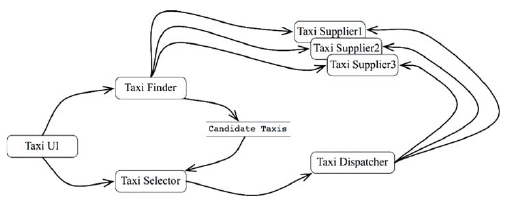
\includegraphics{Taxi system.png}
            \caption*{Figura 5.1: Servicios organizados para implementar el sistema de agregación de taxis (Martin, 2018)}
            \label{fig:Figura5.1}
        \end{figure}

        \begin{table}[H]
            \centering
            \begin{tabular}{|l|p{10cm}|}
                \toprule
                Servicio&Funcionalidad\\
                \midrule
                TaxiUI&Lidia con los clientes, quienes usan dispositivos móviles para ordenar taxis\\
                TaxiFinder&Busca en los inventarios de varios TaxiSuppliers y determina cuáles taxis son posibles candidatos para el usuario\\
                TaxiSelector& Toma los criterios del usuario en cuanto al costo, tiempo, lujo, entre otros y selecciona un taxi apropiado de entre los candidatos y le entrega ese taxi al TaxiDispatcher\\
                TaxiDispatcher&Solicita el taxi apropiado\\
                \bottomrule
            \end{tabular}
            \caption*{Tabla 5.2: Funcionalidades de los servicios propuestos para el sistema de agregación de taxi}
            \label{tab:Tabla5.2}
        \end{table}

        Luego de que el sistema ha estado operando por más de un año en el que el equipo de desarrollo ha estado añadiendo nuevas funcionalidades mientras mantienen y operan los servicios, se desea agregar una característica en específico: la entrega de gatitos.

        Esta nueva funcionalidad consiste en que los clientes ordenan gatitos para que sean entregados en sus hogares o en sus lugares de trabajo. Cuando se solicita un gatito, el taxi más cercano será seleccionado para recoger al minino de uno de los puntos de recogida repartidos por la ciudad y entregarlo en la dirección apropiada.

        Surgen los siguientes inconvenientes:

        \begin{itemize}
            \item Algunos proveedores de taxis pueden no estar de acuerdo con participar en esta nueva oferta.
            \item Algunos conductores pueden ser alérgicos a los gatos, por lo que no podrán ser seleccionados por este servicio.
            \item Algunos clientes pueden ser alérgicos a los gatos, así que el vehículo que ha sido utilizado para entregar gatitos en los últimos tres días no debería ser seleccionado por los clientes que han declarado tales alergias.
        \end{itemize}

        Al observar el diagrama de servicios, todos deben cambiar para implementar la nueva funcionalidad.

        \subsection{La causa del problema}

        La solución de dividir el sistema en servicios basados en verbos o entidades funcionales (como TaxiFinder o TaxiSelector) llevó a este problema ya que la nueva funcionalidad de entregar gatos requiere un cambio coordinado en todos los servicios ya existentes, esto debido a los inconvenientes descritos en el problema: Como algunos proveedores pueden no estar de acuerdo con participar en la nueva oferta, ese TaxiSupplier no puede estar disponible y TaxiFinder no puede elegirlo, así como de los disponibles, no puede elegir a conductores alérgicos, TaxiSelector debe tener en cuenta, además de los criterios, las alergias de los clientes, TaxiDispatcher debe mandar el taxi adecuado con todas estas restricciones y, sobre todo, TaxiUI debe implementar el mecanismo para que los clientes puedan introducir las posibles alergias.

        \subsection{Solución usando principios DDD y Arquitectura Onion/Clean}

        Si el sistema se hubiese diseñado usando los principios SOLID y se le diese una estructura de componentes, podría haberse logrado el objetivo de que los nuevos componentes puedan agregarse sin cambiar los componentes existentes dentro del servicio (Martin, 2018). Es decir crear un conjunto de clases que podrían ser polimórficamente expansibles para manejar nuevas funcionalidades. (Ver \hyperref[fig:Figura5.3]{Figura 5.3})

        \begin{figure}[H]
            \centering
            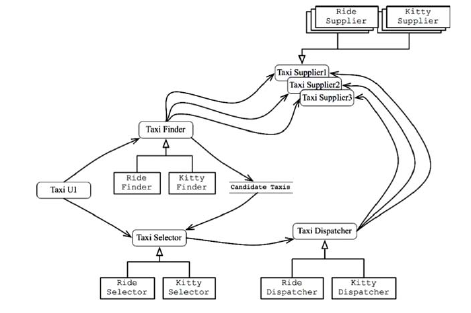
\includegraphics{Solucion Kitty Problem.png}
            \caption*{Figura 5.3: Cada componente tiene su propio diseño de componente interno, permitiendo que nuevas funcionalidades sean añadidas como nuevas clases derivadas (Martin, 2018)}
            \label{fig:Figura5.3}
        \end{figure}

        La solución que se propone es la siguiente:

        Los servicios que ya teníamos (exceptuando TaxiUI) pasarán a ser clases abstractas (o implementación equivalente dependiendo del lenguaje de programación utilizado), que servirán de plantilla para los dos nuevos componentes: Rides y Kittens.

        Gran parte de la lógica original de servicios es preservada, sin embargo, toda la lógica de paseos se extrae en el componente Rides y la nueva funcionalidad para gatitos se pone en el componente Kittens. Ambos componentes sobrescriben las clases base abstractas en el componente original.

        \subsection{Principio Abierto/Cerrado y papel de los Adaptadores}

        Los dos nuevos componentes siguen la Regla de Dependencia y las clases que implementan esas funcionalidades son creadas por factorías bajo el control de la UI, en este esquema, cuando la funcionalidad de gatitos es implementada, TaxiUI debe cambiar, pero nada más. De hecho, solo se añade un nuevo archivo al sistema que se carga dinámicamente en tiempo de ejecución. Esto evidencia que se cumple el principio Abierto/Cerrado, que plantea que una entidad de software debe quedarse abierta para su extensión, pero cerrada para su modificación (Martin, 2018).

        En este escenario, los adaptadores se encargan de traducir una determinada petición que provenga de una capa externa (la UI, por ejemplo), al caso de uso específico de Rides o Kittens, que aplica las reglas de negocio específicas y, en caso de que se requiera de algún proveedor externo de transporte, interactúa con él por medio de una interfaz definida. Es decir, los adaptadores permiten conectar estas extensiones con el resto del sistema, respetando los límites de la arquitectura.

        \section[Evaluación de la Arquitectura N-Capas frente a Requisitos de Atributos de Calidad]{Pregunta 6: Evaluación de la Arquitectura N-Capas frente a Requisitos de Atributos de Calidad}
        \subsection{Pregunta}

        La Arquitectura N-Capas es criticada por su bajo rendimiento en características como ``Agilidad general'', ``Facilidad de despliegue'' y ``Escalabilidad'' (Richards, 2015). Un estudiante propone que, con el uso de capas abiertas (open layers) y técnicas como ``fast-lane reader'', se pueden mitigar estos problemas.

        Analice esta afirmación. ¿Cómo afecta la introducción de capas abiertas al principio de Aislamiento de Capas y a la mantenibilidad a largo plazo? ¿Por qué la solución de capas abiertas puede llevar a un ``sinkhole anti-pattern'' y qué dice la regla del 80/20 sobre esto? Finalmente, explique por qué, para un sistema con requisitos de alta escalabilidad y agilidad, una arquitectura como la Hexagonal o la Limpia, que se basan en los principios de DDD y desacoplamiento, son inherentemente más adecuadas que una Arquitectura N-Capas, incluso con optimizaciones.

        \subsection{Breve introducción}

        La Arquitectura N-Capas (también llamada layered architecture o n-tier) organiza los componentes en capas horizontales (presentación, negocio, persistencia, base de datos) y suele implementarse como una aplicación monolítica: todas las capas se empaquetan y despliegan como una sola unidad. Esa naturaleza monolítica es la raíz de las críticas que recibe.
        
        \subsubsection*{Agilidad general}
        
        En N-Capas, los cambios pequeños pueden aislarse, pero los cambios grandes son difíciles debido a la naturaleza monolítica del patrón. Cualquier modificación que cruce capas obliga a tocar y probar varios módulos, lo que ralentiza la evolución del software.
        
        \subsubsection*{Facilidad de despliegue}
        
        El despliegue se vuelve problemático en aplicaciones grandes porque todo el monolito debe recompilarse, probarse y desplegarse como una sola unidad. No se pueden desplegar de forma independiente solo las capas o componentes modificados, lo que genera ciclos de despliegue lentos y arriesgados. La estructura monolítica de N-Capas limita la agilidad y convierte el despliegue en un cuello de botella.
        
        \subsubsection*{Escalabilidad}
        
        Para atender un aumento de carga, normalmente hay que escalar toda la aplicación (o grandes porciones de ella) aunque solo una parte necesite más recursos. No se puede escalar de forma selectiva la capa que realmente lo requiere, lo que es ineficiente y encarece el crecimiento.

        Richards (2015) no dice que N-Capas sea ``malo'' en términos absolutos; lo presenta como un patrón con trade-offs: es simple, fácil de entender y muy extendido, pero sacrifica agilidad, despliegue y escalabilidad frente a estilos distribuidos como microservicios o arquitecturas orientadas a eventos.
        
        Técnicas como el ``fast-lane reader'' o el uso de capas abiertas pueden mitigar estos problemas atacando desde un ángulo de eficiencia en el flujo de las peticiones, no desde la estructura de despliegue.

        \subsection{Análisis de agilidad, facilidad de despliegue y escalabilidad aplicando estas técnicas}
        
        \subsubsection*{Agilidad}
        
        Las capas abiertas y el Fast-Lane Reader reducen el ``radio de impacto'' de ciertos cambios. Si una operación de lectura simple no necesita pasar por la capa de negocio, modificarla o corregirla no requiere tocar esa capa, agilizando el ciclo de cambio para ese tipo de funcionalidad.
        
        \subsubsection*{Facilidad de despliegue}
        
        El despliegue sigue siendo monolítico (todo el artefacto se empaqueta junto), por lo que estas técnicas no resuelven el problema de fondo: no permiten desplegar de forma independiente solo la capa o el componente modificado. Sin embargo, al evitar cambios innecesarios en las capas intermedias, pueden reducir la frecuencia con la que un cambio obliga a recompilar y redesplegar todo el monolito, ofreciendo una mejora marginal, no estructural.
        
        \subsubsection*{Escalabilidad}
        
        El Fast-Lane Reader mejora el rendimiento al eliminar el procesamiento innecesario en las capas intermedias para lecturas simples. Al reducir la carga de trabajo por petición, disminuye la presión total sobre el sistema, lo que puede traducirse en una necesidad menor (o más tardía) de escalar el conjunto. No obstante, si la carga de esas lecturas simples crece exponencialmente, la solución seguiría siendo escalar el monolito completo, ya que la técnica no aísla la capa de datos para un escalado independiente.

        Las capas abiertas y el Fast-Lane Reader son ``válvulas de escape'' que optimizan el flujo de las peticiones y evitan trabajo innecesario, lo que se traduce en mejoras de eficiencia y tiempos de respuesta. Sin embargo, no son una solución a la crítica estructural de Richards.
        
        \subsection{Impacto de la introducción de capas abiertas en el Principio de Aislamiento de Capas}
        
        La introducción de capas abiertas en una arquitectura N-Capas genera un trade-off fundamental: se gana en rendimiento y eficiencia, pero se sacrifica el aislamiento entre capas, lo que tiene un impacto directo y negativo en la mantenibilidad a largo plazo.

        El principio de aislamiento de capas busca que los cambios en una capa no afecten a las demás, siempre que los contratos (interfaces) se mantengan estables. En una arquitectura de capas cerradas, este principio se respeta estrictamente porque una capa solo puede comunicarse con la inmediatamente inferior, lo que reduce las dependencias y promueve la independencia entre capas.

        Las capas abiertas rompen este principio. Al permitir que una capa superior omita capas intermedias y acceda directamente a cualquier capa inferior (por ejemplo, la de persistencia), se crean dependencias directas que de otro modo no existirían. Esto rompe la encapsulación de las capas intermedias y genera un mayor acoplamiento en todo el sistema. La estructura deja de ser una cadena de dependencias unidireccional y estricta para convertirse en una red con múltiples atajos, donde los límites entre capas se vuelven porosos.

        \subsection{Impacto de la introducción de capas abiertas en la mantenibilidad}
        La mantenibilidad a largo plazo se ve comprometida como consecuencia directa de la pérdida de aislamiento.

        Beneficio a corto plazo (Rendimiento): La razón principal para usar capas abiertas es el rendimiento. Al evitar la sobrecarga de procesamiento (y a veces de red) de las capas intermedias, se reduce la latencia de las peticiones.

        Coste a largo plazo (Mantenibilidad): Este beneficio inicial se paga con un alto precio en mantenibilidad. La razón es que el mayor acoplamiento hace que el sistema sea más frágil. Un cambio en la capa de persistencia (por ejemplo, en un esquema de base de datos) puede romper el código de la capa de presentación que accedía a ella directamente, ya que esta capa ya no está protegida por la capa de negocio intermedia. Esto obliga a cambiar y probar en más lugares cada vez que se modifica algo, lo que dificulta la evolución del sistema y aumenta el riesgo de introducir errores en cascada. La arquitectura, que era fácil de entender, se vuelve más compleja y difícil de gestionar con el tiempo.

        \subsection{La relación entre las capas abiertas, el Sinkhole Antipattern y la regla del 80/20}

        El Architecture Sinkhole Antipattern ocurre cuando una petición atraviesa múltiples capas que se limitan a reenviarla, sin realizar lógica de negocio, validaciones o transformaciones que justifiquen ese procesamiento. Esto introduce sobrecarga y complejidad sin aportar suficiente valor.

        Las capas abiertas constituyen una posible solución a este problema, ya que permiten que determinadas peticiones omitan las capas intermedias que no necesitan. Sin embargo, esta decisión implica un compromiso: aunque puede mejorar el rendimiento, reduce el aislamiento entre capas y aumenta el acoplamiento, lo que puede dificultar la mantenibilidad a largo plazo.

        Richards propone utilizar la regla del 80/20 como una heurística para evaluar la conveniencia de una arquitectura en capas. Si aproximadamente el 20\% de las peticiones son simples pasamanos y el 80\% contienen lógica relevante, la arquitectura puede seguir siendo adecuada. En cambio, si la mayoría de las peticiones atraviesan las capas sin obtener un valor significativo de ellas, conviene considerar la apertura selectiva de capas o la adopción de un estilo arquitectónico más apropiado para el problema.

        Por tanto, la decisión no consiste en abrir todas las capas indiscriminadamente, sino en evaluar el comportamiento real de las peticiones y equilibrar el rendimiento con el aislamiento, el acoplamiento y la mantenibilidad.

        \subsection{Por qué las arquitecturas Hexagonal y Limpia pueden ser más adecuadas para sistemas con requisitos elevados de agilidad y escalabilidad}

        En una arquitectura N-Capas tradicional, las dependencias suelen dirigirse desde las capas superiores hacia las inferiores. Cuando la lógica de negocio depende directamente de detalles de persistencia o de tecnologías concretas, los cambios en la infraestructura pueden propagarse hacia el dominio y dificultar su evolución.

        Las arquitecturas Hexagonal y Limpia aplican el principio de inversión de dependencias para proteger la lógica de negocio de los detalles externos. En estos estilos, el dominio define las abstracciones necesarias y la infraestructura las implementa mediante adaptadores. De esta manera, es posible sustituir tecnologías o modificar mecanismos de entrada y salida con menor impacto sobre la lógica central.

        Este desacoplamiento favorece la mantenibilidad, la testabilidad y la agilidad de evolución. Además, facilita la organización del sistema en módulos que pueden evolucionar de forma más independiente.

        No obstante, estas arquitecturas no garantizan por sí mismas una mayor escalabilidad ni el despliegue independiente de sus componentes, ya que también pueden implementarse como monolitos. Para conseguir escalado independiente se necesitan decisiones adicionales sobre modularización, distribución y despliegue.

        En conclusión, Hexagonal y Limpia pueden resultar más adecuadas cuando la prioridad es proteger el dominio y facilitar la evolución del sistema. Si la escalabilidad es un requisito dominante, su combinación con una estrategia apropiada de modularización y despliegue puede proporcionar ventajas frente a una arquitectura N-Capas tradicional, sin que ello implique que esta última sea siempre inadecuada.
        \section{Bibliografía}
        \begin{itemize}
            \item Cockburn, A. (2005). Hexagonal Architecture (Ports and Adapters). Consultado en: \url{https://alistair.cockburn.us/hexagonal-architecture/}
            \item De la Torre Llorente, C., Zorrilla Castro, U., Ramos Barroso, M. A., \& Calvarro Nelson, J. (2010). Guía de Arquitectura N-Capas orientada al Dominio con .NET 4.0 (Borrador). Microsoft Ibérica.
            \item Evans, E. (2003). Domain-Driven Design: Tackling Complexity in the Heart of Software. Addison-Wesley Professional.
            \item Martin, R. C. (2018). Clean Architecture: A Craftsman's Guide to Software Structure and Design. Prentice Hall.
            \item Palermo, J. (2008). The Onion Architecture. Consultado en: \url{https://jeffreypalermo.com/2008/07/the-onion-architecture-part-1/}
            \item Richards, M. (2015). Software Architecture Patterns. O'Reilly Media.
            \item Richards, M., \& Ford, N. (2020). Fundamentals of Software Architecture: An Engineering Approach. O'Reilly Media.
        \end{itemize}

        \section{Declaración de uso de IA}

        Para la elaboración de este seminario, el equipo en general utilizó las herramientas ChatGPT y DeepSeek con el propósito de asistir en la generación de ejemplos ilustrativos, la optimización del texto y la corrección ortográfica. Todo el contenido generado fue revisado, verificado y adaptado por el equipo, quien asume la responsabilidad final del documento.
\end{document}